\documentclass{beamer}
\usetheme{Frankfurt}

\usepackage[utf8]{inputenc}
\usepackage[spanish,es-noquoting]{babel}
%\usepackage[unicode=true]{hyperref}
\usepackage{amsmath}
\usepackage{color, colortbl}
\usepackage{amsfonts}
\usepackage{amssymb}
\usepackage{graphicx}
\usepackage{subfig}
\usepackage{url}
\usepackage{booktabs}
\usepackage{adjustbox}
\usepackage{tikz}
\usepackage{rotating} 
\usepackage{tkz-graph}
\usetikzlibrary{arrows,automata,fit}
\usetikzlibrary{calc,positioning,shapes.geometric}
\usetikzlibrary{shapes}
\usetikzlibrary{er}

\definecolor{LRed}{rgb}{0.0, 0.0, 1.0}

\newcounter{sauvegardeenumi}
\newcommand{\asuivre}{\setcounter{sauvegardeenumi}{\theenumi}}
\newcommand{\suite}{\setcounter{enumi}{\thesauvegardeenumi}}
\newcommand{\arquitectura}{
	\begin{tikzpicture}[database/.style={
		cylinder,
		cylinder uses custom fill,
		cylinder body fill=white,
		cylinder end fill=white,
		shape border rotate=90,
		aspect=0.25,
		draw
	}]
			% Base de datos
			\node[database, scale=2] at (5,2.25) (mysql) {MySQL};
				
			% Parser
			\draw (1,1.5) rectangle (3,3.5) node[midway] {PARSER};
				
			% API REST
			\draw (7,1.5) rectangle (9,3.5) node[midway] {API REST};
				
			% APP Angular
			\draw (5,-2.5) rectangle (9,-4.5) node[midway] {Aplicación AngularJS};
				
			% Nube
			\node[cloud, cloud puffs=15, cloud ignores aspect, minimum width=3cm, minimum height=2cm, align=center, draw] (cloud) at (-3, 2.5) {lfp.es};
				
			% Backend
			\draw (0,0) rectangle (10,5);
				
			% Frontend
			\draw (0,-5) rectangle (10,-1);
				
			% Flechas
				
			% Nube - Parser 
			\draw [<-] (1, 2.5) -- node[anchor=south] {HTTP}    (-1.5,2.5);
				
			% Parser - MySQL
			\draw [->] (3, 2.50)   -- node {}  (3.3,2.50);
				
			% API REST - MySQL
			\draw [->] (6.7, 2.25)   -- node {}  (7.00,2.25);
			\draw [<-] (6.7, 2.75)   -- node {}  (7.00,2.75);
				
			% API REST - AngularJS
			\draw [->] (7.5, 1.5)   -- node {}      (7.5,-2.5);
			\draw [<-] (8.5, 1.5)   -- node[anchor=west] {REST}  (8.5,-2.5);
				
			% Backend
			\node at (5,4.75) {\textbf{BACKEND}};
				
			% Frontend
			\node at (5,-1.25) {\textbf{FRONTEND}};

	\end{tikzpicture}}
\usepackage{amsmath}
\usepackage{xparse}
\usepackage{amsthm}
\usepackage{tikz}

% Seno
\def\sen{\mathop{\mbox{\normalfont sen}}\nolimits}

% Seno hiperbólico
\def\senh{\mathop{\mbox{\normalfont senh}}\nolimits}

% Arcoseno
\def\arcsen{\mathop{\mbox{\normalfont arcsen}}\nolimits}

% Gradiente
\def\grad{\mathop{\mbox{\normalfont grad}}\nolimits}

% Argumento principal
\def\Arg{\mathop{\mbox{\normalfont Arg}}\nolimits}

% Logaritmo complejo
\def\Log{\mathop{\mbox{\normalfont Log}}\nolimits}

% Rotacional
\def\rot{\mathop{\mbox{\normalfont rot}}\nolimits}

% Divergencia
\def\diver{\mathop{\mbox{\normalfont div}}\nolimits}

% Longitud
\def\longi{\mathop{\mbox{\normalfont long}}\nolimits}

% Índice de una curva
\def\ind{\mathop{\mbox{\normalfont Ind}}\nolimits}

% Rango de una matriz
\def\rang{\mathop{\mbox{\normalfont rang}}\nolimits}

% Norma
\newcommand{\norm}[1]{\lVert #1 \rVert}

% Derivada parcial
\newcommand{\derpar}[1]{\dfrac{\partial}{\partial #1}}

% Derivada parcial con función
\newcommand{\derparcial}[2]{\dfrac{\partial #1}{\partial #2}}

% Derivada parcial de orden n con funcion
\newcommand{\derparcialn}[3]{\dfrac{\partial^{#3} #1}{\partial #2^{#3}}}

% Integral doble en [a,b] x [c,d]
\newcommand{\intdob}[4]{\displaystyle \int_{#1}^{#2} \int_{#3}^{#4}}

% Integral triple en [a,b] x [c,d] x [e,f]
\newcommand{\inttri}[6]{\displaystyle \int_{#1}^{#2} \int_{#3}^{#4} \int_{#5}^{#6}}

% Números complejos
\def\C{\ensuremath{\mathbb{C}}}

% Números reales
\def\R{\ensuremath{\mathbb{R}}}

% Números racionales
\def\Q{\ensuremath{\mathbb{Q}}}

% Números enteros
\def\Z{\ensuremath{\mathbb{Z}}}

% Números naturales
\def\N{\ensuremath{\mathbb{N}}}

% Teorema
\newtheorem{teo}{Teorema}

% Corolario
\newtheorem{cor}{Corolario}

% Proposición
\newtheorem{prop}{Proposición}

% Lema
\newtheorem{lema}{Lema}

% Definición
\newtheorem{defi}{Definición}

% Observaciones
\newtheorem*{obs}{Observaciones}

\newtheorem*{ob}{Observación}

\newtheorem*{nota}{Nota}

\newtheorem*{problema}{Problema}

\newtheorem*{pregunta}{Pregunta}

\newtheorem{ejemplo}{Ejemplo}

\NewDocumentCommand{\overarrow}{O{=} O{\uparrow} m}{%
  \overset{\makebox[0pt]{\begin{tabular}{@{}c@{}}#3\\[0pt]\ensuremath{#2}\end{tabular}}}{#1}
}
\NewDocumentCommand{\underarrow}{O{=} O{\downarrow} m}{%
  \underset{\makebox[0pt]{\begin{tabular}{@{}c@{}}\ensuremath{#2}\\[0pt]#3\end{tabular}}}{\ensuremath{#1}}
}

\newcommand{\contradiction}{%
\begin{tikzpicture}[rotate=45,x=0.5ex,y=0.5ex]
\draw[color=red, line width=.1ex] (0,2) -- (3,2) (0,1) -- (3,1) (1,3) -- (1,0) (2,3) -- (2,0);
\end{tikzpicture}
}


\title{TFG Matemáticas (6 ECTS):\\ Modelos predictivos en rankings.\\ TFG Informática (15 ECTS):\\ Diseño e implementación de modelos de predicción para la Liga BBVA.}
\author{Javier Jiménez del Peso}
\institute[URJC]{
\includegraphics[scale=0.3]{images/logoURJC.jpg}}
\date{\today}


\begin{document}

	\begin{frame}
		\titlepage
	\end{frame}

	\begin{frame}{Índice}
		\tableofcontents[hideallsubsections]
	\end{frame}

	\section{Introducción}
	\subsection{a}
	\begin{frame}
		\begin{center}
			\Huge\textbf{\textsf{\textcolor{blue}{Introducción y objetivos}}}
		\end{center}
	\end{frame}
	
	\begin{frame}{Introducción}
		Los rankings forman parte de nuestra vida cotidiana:
		
		\begin{itemize}
			\item De países por PIB			
			\item De líderes políticos
			\item De universidades
			\item De éxitos musicales del momento
			\item De películas más taquilleras del año
			\item Deportivos: FIFA, ATP, etc. 
		\end{itemize}
	\end{frame}	
	
	\begin{frame}{Introducción}
		\begin{figure}
			\centering
			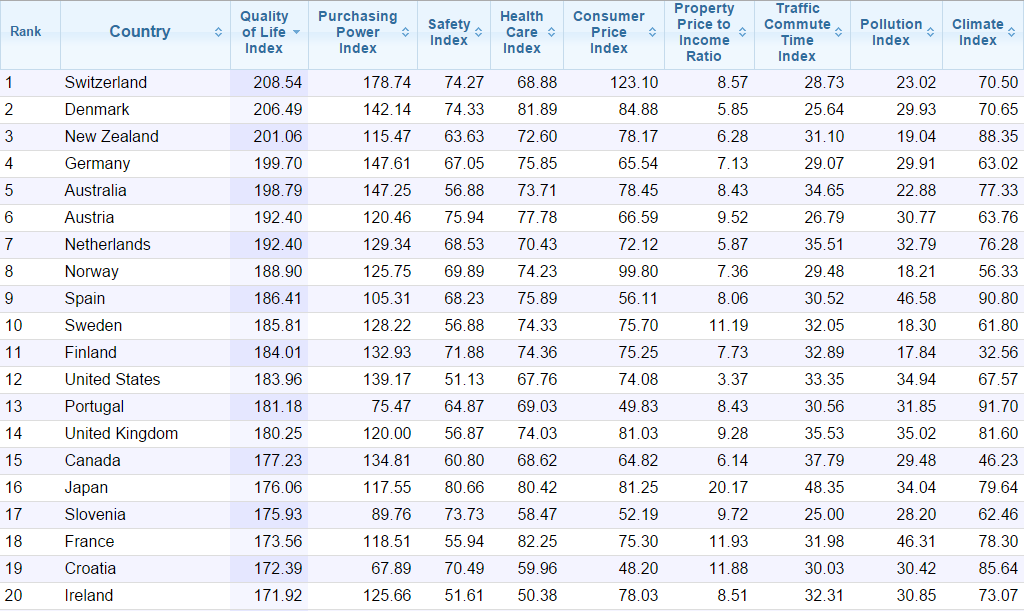
\includegraphics[width=0.9\linewidth]{images/ranking_calidad_vida.png}
			\caption{Ranking de países por calidad de vida (2016) \url{www.numbeo.com/quality-of-life/rankings_by_country.jsp}}
		\end{figure}
	\end{frame}

	\begin{frame}{Introducción}
		\begin{figure}
			\centering
			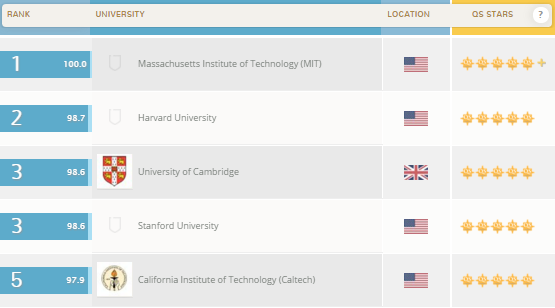
\includegraphics[width=0.85\linewidth]{images/ranking_universidades.png}
			\caption{Ranking de universidades (2015/16) \url{http://www.topuniversities.com/university-rankings/world-university-rankings/2015}}
		\end{figure}
	\end{frame}
	
	\begin{frame}{Introducción}
		\begin{figure}
			\centering
			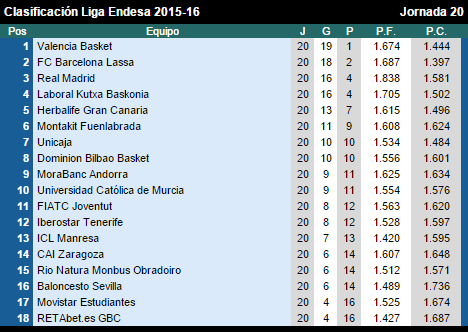
\includegraphics[width=0.80\linewidth]{images/ranking_acb.png}
			\caption{Ranking de la ACB (temporada 2015/16) \url{http://www.acb.com/resulcla.php}}
		\end{figure}
	\end{frame}

	\begin{frame}{Objetivos}
		\begin{itemize}
			\item Conocer distintas herramientas para trabajar con rankings y ratings.			
			\item Proponer varios modelos de predicción de resultados deportivos.
			\item Implementar un módulo que obtenga la predicción de resultados de los partidos y el ranking final para la próxima jornada de la Liga BBVA de fútbol.  
			\item Analizar y comparar los resultados obtenidos por los distintos modelos.
		\end{itemize}
	\end{frame}
	
	\begin{frame}{Tareas realizadas en el proyecto de Matemáticas}
	\begin{itemize}
		\item Revisión bibliográfica de conceptos y herramientas para trabajar con rankings. Libro principal:\\
		 \textit{Who's \#1? The science of rating and ranking},\\ 
		 A. N. Langville, C. D. Meyer.
		\item Revisión bibliográfica de modelos de predicción de resultados deportivos: \\
		\begin{itemize}
			\item ``Sports forecasting: A comparison of the forecast accuracy of prediction markets, betting odds and tipsters'', \textsc{M.Spann, B.Skiera}.
			\item ``A new model to forecast the results of matches based on hybrid neural networks in the soccer rating system'', \textsc{T.Cheng, D.Cui, Z.Fan, J.Zhou, S.Lu}.
			\item ``Forecasting Indian Premier League Results Using Time Series Analysis'', \textsc{G.Hiranandani, J.Shitole, N.Kundu, N.Maurya, R.Grover}.
		\end{itemize}
		\item Desarrollo de dos nuevos modelos de predicción y su combinación.
	\end{itemize}
	\end{frame}

	\begin{frame}{Tareas realizadas en el proyecto de Informática}
		\begin{itemize}
			\item Desarrollo de un módulo de predicción de resultados de partidos y del ranking final para la próxima jornada de la Liga BBVA de fútbol.
			\item Entrenamiento y validación de los modelos.
			\item Análisis y comparación de resultados. 
		\end{itemize}
	\end{frame}

	\section{Conceptos sobre rankings}
	\subsection{b}
	\begin{frame}
		\begin{center}
			\Huge\textbf{\textsf{\textcolor{blue}{Conceptos básicos sobre rankings}}}
		\end{center}
	\end{frame}	
	
	\begin{frame}{Rankings}
		\begin{defi} 
			Un \textbf{ranking} de tamaño n es una permutación de números naturales desde 1 hasta n, es decir, se trata de una biyección $r: \xi \rightarrow \xi$ donde $\xi = \{1,...,n\}$ con $n \in \mathbb{N}$ es el conjunto de elementos a ordenar.
		\end{defi}
		
		\begin{ejem}
			Ejemplo de ranking.\\
			$$\begin{array}{ccc}
			\begin{array}{c}
			\text{A}\\
			\text{B} \\
			\text{C} \\
			\text{D} \\
			\end{array} & \left(\begin{array}{c}
			2\\
			4\\
			1\\
			3
			\end{array} \right)
			\end{array}  $$	
		\end{ejem}	
	\end{frame}

	\begin{frame}{Ratings}
		\begin{defi} 
			Un \textbf{rating} es una lista de puntuaciones numéricas, una por cada elemento, es decir, $\tilde{r}: \xi \rightarrow \mathbb{R}$ donde $\xi = \{1,...,n\}$ con $n \in \mathbb{N}$ es el conjunto de todos los elementos.
		\end{defi}
		
		\begin{ejem}
			Ejemplo de rating.\\
			$$\begin{array}{ccc}
			\begin{array}{c}
			\text{A}\\
			\text{B} \\
			\text{C} \\
			\text{D} \\
			\end{array} & \left(\begin{array}{c}
			9\\
			3\\
			12\\
			7
			\end{array} \right)
			\end{array} $$ 	
		\end{ejem}	
		Ordenando un rating, siempre se obtiene un ranking.
	\end{frame}

	\begin{frame}{Métodos para obtener rankings}
		Consiste en la creación de nuevos rankings en base a diferentes estadísticas aplicando distintos métodos.
		\begin{itemize}
			\item \textbf{Método de Massey.} Está basado en la teoría de mínimos cuadrados y hace uso de la diferencia de puntos de los equipos.
			\item \textbf{Método de Colley.} Hace uso del porcentaje de victorias y derrotas de los equipos.
			\item \textbf{Método de Keener.} Hace uso de cualquier estadística no negativa de los partidos (partidos ganados, puntos, triples, yardas,...).
			\item \textbf{Método de ataque-defensa.} Consiste en asignar a cada equipo dos ratings, uno de ataque y otro de defensa que combinaremos para obtener el ranking final.
		\end{itemize}
	\end{frame}

	\begin{frame}{Métodos de agregación de rankings}
		Consiste en la combinación de diversos rankings para obtener uno más robusto.
		\begin{itemize}
			\item \textbf{Ranking promedio.} Consiste en hacer la media aritmética de las posiciones que ocupa cada elemento en los rankings.
			\item \textbf{Suma de borda.} Por cada ranking, cada elemento recibe una puntuación igual al número de elementos que supera. Posteriormente se suman para cada elemento.
			\item \textbf{Método óptimo de agregación.} Consiste en resolver un problema de optimización que pretende maximizar las concordancias entre los rankings de entrada.
		\end{itemize}
	\end{frame}
	
	\begin{frame}{Métodos de comparación de rankings}
		Se usan con el objetivo de estudiar el grado de coincidencia entre dos rankings.
		\begin{block}{Tau de Kendall}
			\begin{itemize}
				\item Si tenemos dos rankings $r_{1}$ y $r_{2}$, diremos que el par de elementos $(i,j)$ es concordante si la posición relativa entre ambos en las dos listas es la misma, es decir, $i$ aparece por encima de $j$ o $j$ aparece por encima de $i$ en ambos rankings.
				\item Dados dos rankings $r_{1}$ y $r_{2}$, el valor de la \textbf{Tau de Kendall} $\tau(r_{1},r_{2})$ se puede hallar como
				\begin{equation*}
				\tau = \dfrac{n_{c} - n_{d}}{n(n-1)/2},
				\end{equation*}
				donde $n_{c}$ es el número de pares concordantes, $n_{d}$ el de pares discordantes y $n$ el número de ítems de los rankings.  
			\end{itemize}
		\end{block}
	\end{frame}	

	\begin{frame}{Métodos de comparación}
		\begin{block}{Rho de Spearman}
			La \textbf{Rho de Spearman} es la distancia entre dos rankings completos $r_{1}$ y $r_{2}$ de tamaño $n$. 
			\begin{equation} 
			\phi = \sum_{i=1}^{n} \dfrac{|r_{1}(i) - r_{2}(i)|}{min\{r_{1}(i),r_{2}(i)\}}
			\end{equation}
			donde $r_{1}(i)$ es el puesto del equipo $i$ en el ranking $r_{1}$ y $r_{2}(i)$ es el puesto del equipo $i$ en el ranking $r_{2}$.	
		\end{block}		
	\end{frame}	

	\begin{frame}{Métodos de comparación}	
		\begin{ejem}		
			Vamos a calcular la Tau de Kendall y la Rho de Spearman para los siguientes rankings. 	
			$$\begin{array}{ccc}
			\begin{array}{c}
			\text{A}\\
			\text{B} \\
			\text{C} \\
			\text{D} \\
			\end{array} & \left(\begin{array}{c}
			2\\
			4\\
			1\\
			3
			\end{array} \right)& \left(\begin{array}{c}
			1\\
			4\\
			2\\
			3
			\end{array} \right)
			\end{array}$$  \\
			$$ \tau (r_{1},r_{2}) = \dfrac{5-1}{6}=0.6666667$$\\
			$$ \phi (r_{1},r_{2}) = \frac{|2-1|}{1} + 0 + \frac{|1-2|}{1} + 0 = 2$$
		\end{ejem}
	\end{frame}	

	\section{Modelos de predicción}
	\subsection{c}
	\begin{frame}
		\begin{center}
			\Huge\textbf{\textsf{\textcolor{blue}{Modelos de predicción}}}
		\end{center}
	\end{frame}	
	
	\begin{frame}
		\frametitle{Modelos de predicción}
		\textbf{Objetivo}: realizar una predicción de los resultados de los partidos y el ranking final para la próxima jornada de la Liga BBVA.\\
		\ \\
		\begin{itemize}
			\item Predicción de resultados de los partidos: Tres modelos propuestos.
			\begin{itemize}
				\item Probabilidad basada en la posición relativa de los equipos.
				\item Probabilidad basada en la tendencia de cada equipo.
				\item Combinación de los anteriores.
			\end{itemize}
			\item Predicción de ranking final: Usando los resultados de la predicción de los partidos.
		\end{itemize} 
		\ \\
		\textbf{Fase de entrenamiento}: en las primeras 20 jornadas no realizaremos predicciones, solo recogemos datos.
	\end{frame}	
	
	\begin{frame}
		\frametitle{Probabilidad basada en la posición relativa}
		\begin{enumerate}
			\item Calcular la diferencia entre las posiciones de los equipos: 
			\begin{equation*}
				r(a)-r(b) \in [-19,19] \backslash \{0\}
			\end{equation*}
			\item Reescalar al $[0,1]$:
			\begin{eqnarray*}
				\psi: [-19,19] \longrightarrow [0,1] \\
				t \longmapsto \dfrac{t+19}{38}
			\end{eqnarray*}
			\asuivre
		\end{enumerate}
	\end{frame}

	\begin{frame}
		\frametitle{Probabilidad basada en la posición relativa}
		\begin{enumerate}
			\suite
			\item Definir umbrales de victoria para el equipo local, empate y victoria visitante en tres escenarios:
			\begin{itemize}
				\item Primero vs último: $\psi = 0$.
				\item En posiciones consecutivas: $\psi=\frac{20}{38}$.
				\item Último vs primero: $\psi = 1$.
			\end{itemize}    	
			\begin{figure}
				\centering
				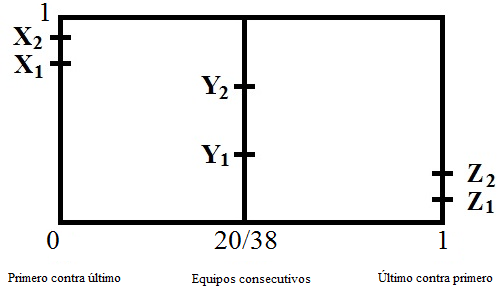
\includegraphics[width=0.6\linewidth]{images/umbrales.png}
			\end{figure}	
			Donde los valores $X_{1},X_{2},Y_{1},Y_{2},Z_{1},Z_{2} \in [0,1]$ nos darán la probabilidad de que gane el equipo local, el visitante o empaten en los tres casos contemplados.
			\asuivre
		\end{enumerate}		
	\end{frame}

	\begin{frame}
		\frametitle{Probabilidad basada en la posición relativa}	
		Por ejemplo, para el caso en que el equipo $a$ es el primero de la clasificación y el equipo $b$ el último:
		\begin{center}
			$\begin{cases}
			P_{r}(a-b=1)=X_{1}\\
			P_{r}(a-b=X)=X_{2}-X_{1} \ \ \ \ \ \ \ \text{siendo} \ 0 \leq X_{1} \leq X_{2} \leq 1.\\
			P_{r}(a-b=2)=1-X_{2} 
			\end{cases}$\\
		\end{center}
		\ \\
		Razonamiento análogo para los otros dos casos.\\
		\ \\
		Los umbrales se obtienen de un histórico de datos de partidos disputados.
	\end{frame}
	
	\begin{frame}
		\frametitle{Probabilidad basada en la posición relativa}
		\begin{enumerate}
			\suite
			\item Interpolar de forma lineal para el resto de casos.\\
			\ \\
			Tenemos dos funciones $f,g:[0,1] \longrightarrow [0,1]$:\\
			\ \\
			$f(n)= \begin{cases}
			X_{2}+\dfrac{Y_{2}-X_{2}}{\frac{20}{38}}n \ \ \ \ \ \ \ \ \ \ \ \ \text{    si } n\leq \frac{20}{38} \\
			Y_{2}+\dfrac{(n-\frac{20}{38})(Z_{2}-Y_{2})}{1-\frac{20}{38}} \ \ \text{    si } n > \frac{20}{38}
			\end{cases}$
			
			$g(n)= \begin{cases}
			X_{1}+\dfrac{Y_{1}-X_{1}}{\frac{20}{38}}n \ \ \ \ \ \ \ \ \ \ \ \ \text{    si } n\leq \frac{20}{38} \\
			Y_{1}+\dfrac{(n-\frac{20}{38})(Z_{1}-Y_{1})}{1-\frac{20}{38}} \ \ \text{    si } n > \frac{20}{38}
			\end{cases}$    
		\end{enumerate}				
	\end{frame}

	\begin{frame}[label=interp]
		\frametitle{Probabilidad basada en la posición relativa}
		\begin{figure} 
			\centering
			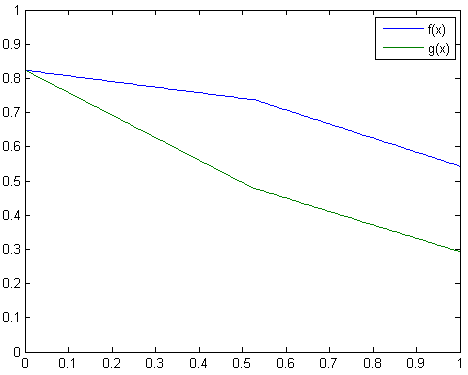
\includegraphics[width=0.65\linewidth]{images/interpolacion.png}
			\caption{Funciones resultantes tras realizar la interpolación usando los umbrales que obtenemos tras analizar los resultados desde la temporada 1990/1991 hasta la actual.}
		\end{figure}			
	\end{frame}

	\begin{frame}
		\frametitle{Probabilidad basada en la tendencia del equipo}
		\begin{itemize}
			\item Para cada equipo trabajaremos con dos secuencias de resultados:
			\begin{itemize}
				\item 5 últimos partidos como local.
				\item 5 últimos partidos como visitante.
			\end{itemize}
		\end{itemize}
		\ \ \ Por ejemplo:	 
		\begin{center}
			\begin{tabular}{|c|c|c|c|c|c|}
				\hline  & t=0 & t=1 & t=2 & t=3 & t=4 \\ 
				\hline local (l)  & 1 & 1 & X & 1 & 2\\ 
				\hline visitante (v) & 2 & 2 & X & 1 & 1\\ 
				\hline 
			\end{tabular} 
		\end{center}
	\end{frame}
	
	\begin{frame}
		\frametitle{Probabilidad basada en la tendencia del equipo}
		De forma que para la jornada siguiente la probabilidad de que el equipo en cuestión gane, empate o pierda será:\\
		
		\begin{center}
			$P_{l}(a - \star=1)=\dfrac{m(0)+m(1)+m(3)}{\sum_{t=0}^{4}m(t)}$\\
			$P_{l}(a - \star=X)=\dfrac{m(2)}{\sum_{t=0}^{4}m(t)}$ \ \ \ \
			$P_{l}(a - \star=2)=\dfrac{m(4)}{\sum_{t=0}^{4}m(t)}$
		\end{center}
		donde $m(t)$ es una función memoria.\\
		\ \\ \ \\
		Razonamiento análogo para la próxima jornada como visitante.
	\end{frame}	
	
	\begin{frame}
		\frametitle{Probabilidad basada en la tendencia del equipo}
		La función memoria servirá para ponderar el resultado de cada partido en función del tiempo que haya transcurrido desde que se disputó.
		\begin{figure}
			\subfloat[Constante]{
				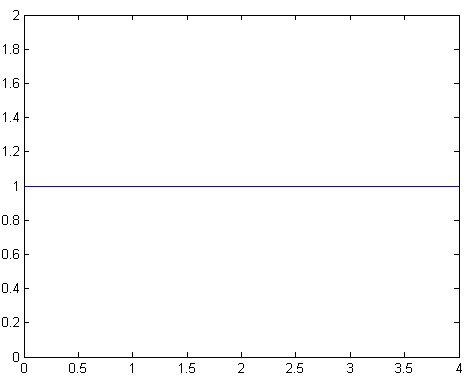
\includegraphics[width=0.33\textwidth]{images/mem1.png}}
			\subfloat[Lineal]{
				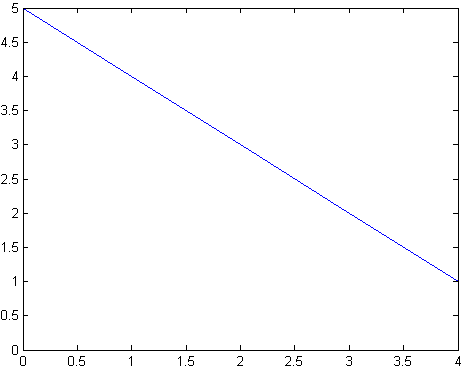
\includegraphics[width=0.33\textwidth]{images/mem2.png}}	
			\subfloat[Exponencial]{
				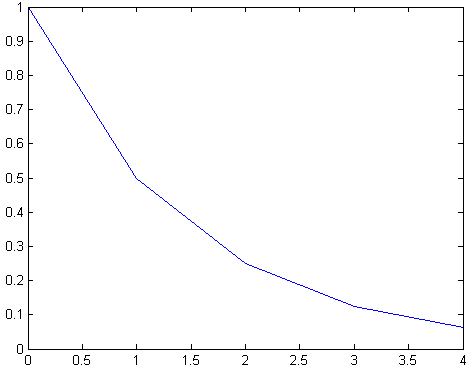
\includegraphics[width=0.33\textwidth]{images/mem3.png}}
			\caption{Tres funciones memoria propuestas.}
		\end{figure} 
	\end{frame}		
	
	\begin{frame}
		\frametitle{Probabilidad basada en la tendencia del equipo}	
		Para pronosticar el resultado del enfrentamiento $a-b$ debemos conjuntar $P_{l}(a - \star)$ con $P_{v}(\star - b)$ de la siguiente forma:
		
	{\tiny $$P_{s}(a-b=1)=
		\left(\begin{array}{ccc}
		P_{l}(a - \star=1) & P_{l}(a - \star=X) & P_{l}(a - \star=2)
		\end{array} \right)
		A_{1}
		\left(\begin{array}{c}
		P_{v}(\star - b=1)\\
		P_{v}(\star - b=X)\\
		P_{v}(\star - b=2)
		\end{array} \right)
		$$	
		$$P_{s}(a-b=X)=
		\left(\begin{array}{ccc}
		P_{l}(a - \star=1) & P_{l}(a - \star=X) & P_{l}(a - \star=2)
		\end{array} \right)
		A_{x}
		\left(\begin{array}{c}
		P_{v}(\star - b=1)\\
		P_{v}(\star - b=X)\\
		P_{v}(\star - b=2)
		\end{array} \right)
		$$
		$$P_{s}(a-b=2)=
		\left(\begin{array}{ccc}
		P_{l}(a - \star=1) & P_{l}(a - \star=X) & P_{l}(a - \star=2)
		\end{array} \right)
		A_{2}
		\left(\begin{array}{c}
		P_{v}(\star - b=1)\\
		P_{v}(\star - b=X)\\
		P_{v}(\star - b=2)
		\end{array} \right)$$
		donde
		$A_{1}=\left(\begin{array}{ccc}
		1 & 1/2 & 1/4\\
		1/2 & 0 & 1/6\\
		1/4 & 1/6 & 0
		\end{array} \right)$,
		$A_{x}=\left(\begin{array}{ccc}
		0 & 1/3 & 1/2\\
		1/3 & 1 & 1/2\\
		1/2 & 1/2 & 0
		\end{array} \right)$ y
		$A_{2}=\left(\begin{array}{ccc}
		0 & 1/6 & 1/4\\
		1/6 & 0 & 1/3\\
		1/4 & 1/3 & 1
		\end{array} \right)$.
		}
	\end{frame}
	
	\begin{frame}
		\frametitle{Combinación de los modelos}
		Ahora contaremos con dos probabilidades: 
		\begin{itemize}
			\item las basadas en la posición relativa: $P_{r}(a-b=1) \ \ P_{r}(a-b=X) \ \ P_{r}(a-b=2)$.
			\item las basadas en la tendencia de cada equipo: $P_{s}(a-b=1) \ \ P_{s}(a-b=X) \ \ P_{s}(a-b=2)$.
		\end{itemize}
		\ \\
		\ \\
		Las conjugamos mediante combinación convexa:
		\begin{center}
			$ P(a-b=1) = \lambda P_{r}(a-b=1) + (1-\lambda) P_{s}(a-b=1)$\\
			$ P(a-b=X) = \lambda P_{r}(a-b=X) + (1-\lambda) P_{s}(a-b=X)$\\
			$ P(a-b=2) = \lambda P_{r}(a-b=2) + (1-\lambda) P_{s}(a-b=2)$
		\end{center}
		debiendo optimizar $\lambda \in [0,1]$ entrenando sobre un histórico de datos.
	\end{frame}

	\section{Descripción informática}
	\subsection{d}
	\begin{frame}
		\begin{center}
			\Huge\textbf{\textsf{\textcolor{blue}{Descripción informática}}}
		\end{center}
	\end{frame}	
		
	\begin{frame}
		\frametitle{Arquitectura}
		\begin{figure}
			\centering
			\resizebox{!}{0.7\textheight}{\arquitectura}
			\caption{Arquitectura de la aplicación}
		\end{figure}
	\end{frame}
	
	\begin{frame}
		\frametitle{Tecnologías usadas}
		\begin{itemize}
			\item Tecnologías del lado del servidor:
		\end{itemize}
		\vspace{-10mm}
		\begin{figure}[htb]
			\centering
			\subfloat{
				
\includegraphics[width=0.11\textwidth]{images/linux.png}}
			\subfloat{
				
\includegraphics[width=0.2\textwidth]{images/apache.png}}
			\subfloat{
				
\includegraphics[width=0.2\textwidth]{images/mysql.png}}
			\subfloat{
				
\includegraphics[width=0.2\textwidth]{images/php.png}}
			\subfloat{
				
\includegraphics[width=0.1\textwidth]{images/composer.png}}
			\subfloat{
				
\includegraphics[width=0.12\textwidth]{images/slim.png}}	
			%\caption{Tecnologías del lado del servidor.}
		\end{figure}
		\begin{itemize}
			\item Tecnologías del lado del cliente:
		\end{itemize}
		\vspace{-8mm}
		\begin{figure}[htb]
			\centering
			\subfloat{
				
\includegraphics[width=0.13\textwidth]{images/html.png}}
			\subfloat{
				
\includegraphics[width=0.13\textwidth]{images/css.png}}
			\subfloat{
				
\includegraphics[width=0.13\textwidth]{images/js.png}}
			\subfloat{
				
\includegraphics[width=0.15\textwidth]{images/bootstrap.png}}
			\subfloat{
				
\includegraphics[width=0.12\textwidth]{images/bower.png}}
			\subfloat{
				
\includegraphics[width=0.18\textwidth]{images/angularjs.png}}
			%\caption{Tecnologías del lado del cliente.}
		\end{figure}
	\end{frame}	
	
	\section{Análisis de resultados}
	\subsection{e}
	\begin{frame}
		\begin{center}
			\Huge\textbf{\textsf{\textcolor{blue}{Análisis de resultados}}}
		\end{center}
	\end{frame}	

	\begin{frame}
		\frametitle{Análisis temporada 2014/2015}
		\begin{itemize}
			\item \textbf{M. Interpolación}:
		\end{itemize}
		Analizando el histórico de datos de partidos desde la temporada 1990/1991 obtenemos los siguientes porcentajes.

		\vspace{-7mm}
		\begin{table}[H]
			\centering
			\begin{tabular}{|c|c|c|c|c|c|c|c|c|}
				\hline
				\multicolumn{3}{|c|}{Primero vs Último} & \multicolumn{3}{|c|}{Consecutivos} & \multicolumn{3}{|c|}{Último vs Primero} \\ \hline
				1 & X & 2 & 1 & X & 2 & 1 & X & 2\\ \hline  			
				0.824 & 0 & 0.176 & 0.478 & 0.259 & 0.263 & 0.292 & 0.250 & 0.458 \\ \hline
			\end{tabular}
		\end{table}
		A partir de estos umbrales realizamos la interpolación (fig \ref{interp}).	
	\end{frame}		
	
	\begin{frame}
		\frametitle{Análisis temporada 2014/2015}
		\begin{itemize}
			\item \textbf{M. Tendencias}: la mejor función memoria es la lineal.
			\begin{figure} 
				\centering
				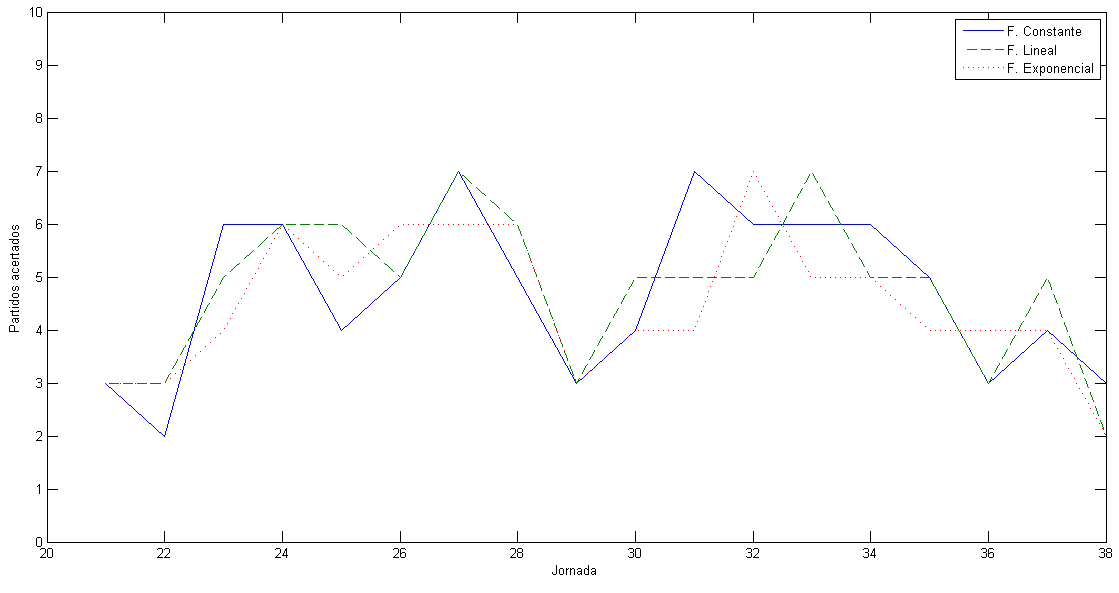
\includegraphics[width=0.85\linewidth]{images/comp_f_m.png}
				\caption{Comparación de resultados obtenidos por las tres funciones memoria.}
			\end{figure}
		\end{itemize}
	\end{frame}	
	
	\begin{frame}
		\frametitle{Análisis temporada 2014/2015}
		\begin{itemize}
			\item \textbf{Combinación}: Optimización de $\lambda$.
			\begin{figure} 
				\centering
				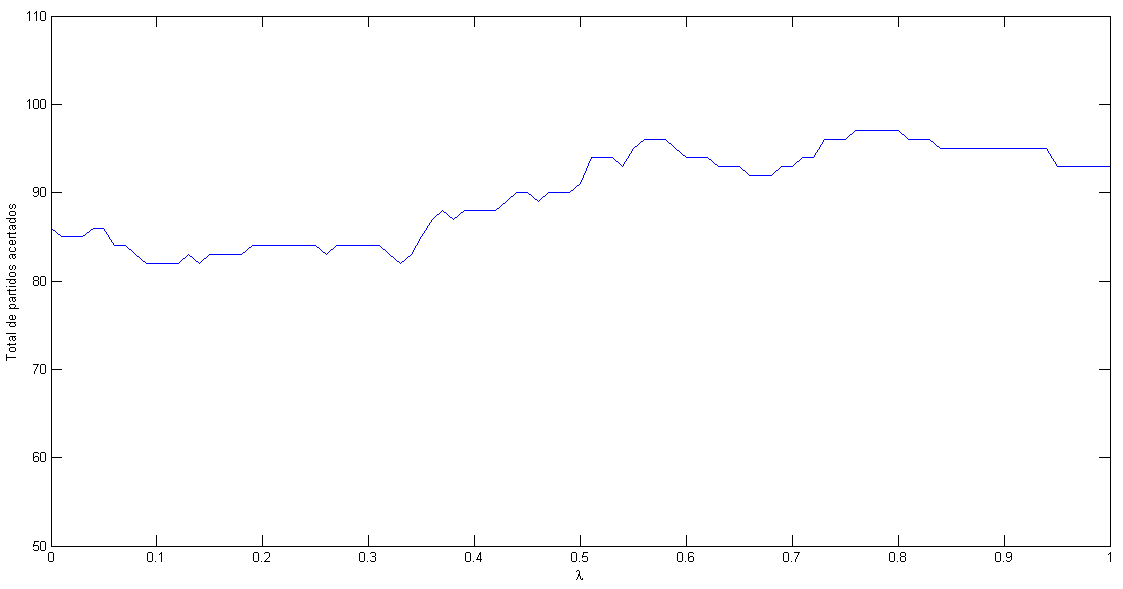
\includegraphics[width=0.85\linewidth]{images/lambda.png}
				\caption{Número total de aciertos según el valor de $\lambda$.}
			\end{figure}
		\end{itemize}
	\end{frame}		

	\begin{frame}
		\frametitle{Análisis temporada 2014/2015}
			\begin{figure} 
				\centering
				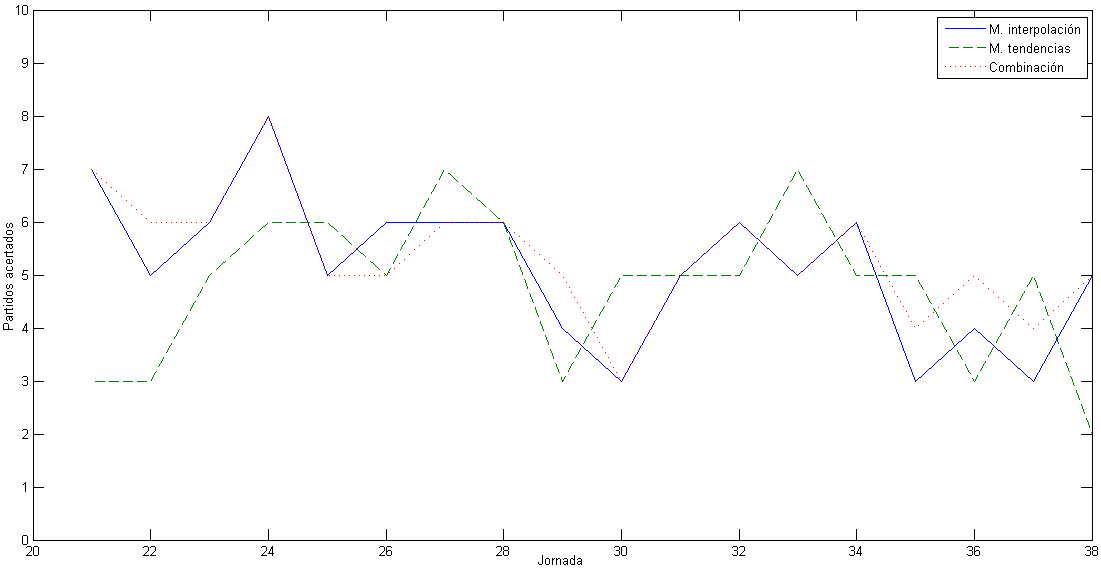
\includegraphics[scale=0.37]{images/comp_mod.png}
				\caption{Comparación de resultados obtenidos por los tres modelos.}
			\end{figure}
	\end{frame}	

	\begin{frame}
		\frametitle{Análisis temporada 2014/2015}
		\begin{figure} 
			\centering
			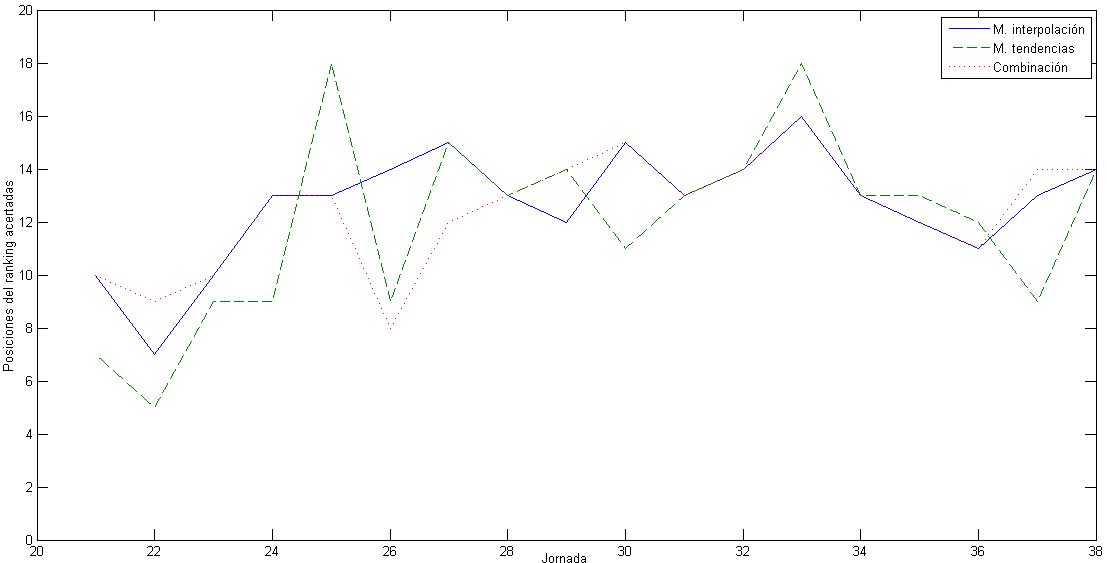
\includegraphics[scale=0.37]{images/comp_mod_2.png}
			\caption{Comparación de posiciones acertadas por los tres modelos.}
		\end{figure}
	\end{frame}	
	
	\begin{frame}
		\frametitle{Análisis temporada 2014/2015}
		\begin{figure} 
			\centering
			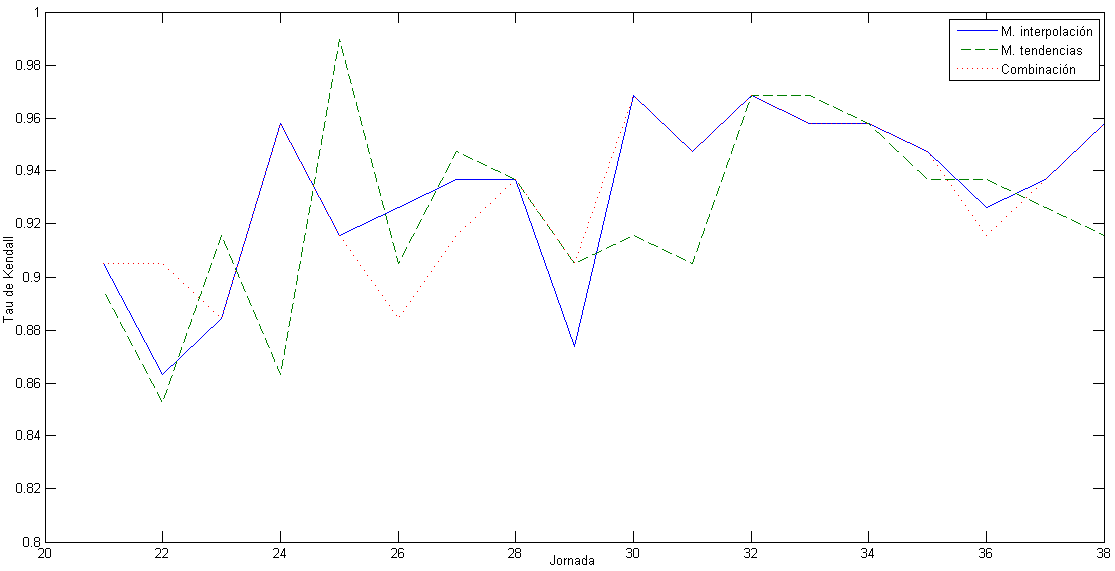
\includegraphics[scale=0.37]{images/comp_mod_3.png}
			\caption{Evolución de la Tau de Kendall de los tres modelos}
		\end{figure}
	\end{frame}	

	\begin{frame}
		\frametitle{Comparación con otras temporadas}
		\begin{block}{Modelo tendencias}
		Comparación de la mejor función memoria:
		\begin{center}
			\begin{tabular}{|c|c|c|c|}
				\hline &  2012/13 &  2013/14 &  2014/15 \\ 
				\hline Partidos & Lineal/Exponencial &  Constante &  Lineal \\ 
				\hline Ranking  &  Lineal &  Exponencial &  Constante \\ 
				\hline 
			\end{tabular} 
		\end{center}			
		\end{block}	
		\begin{block}{Combinación}
			Valores óptimos de $\lambda$:
			\begin{itemize}
				\item Temporada 2012/13: $\lambda=0.72$.
				\item Temporada 2013/14: $\lambda \in [0.83,0.85]$.
				\item Temporada 2014/15: $\lambda \in [0.76,0.80]$.
			\end{itemize}		
		\end{block}
	\end{frame}	

	\section{Conclusión}
	\subsection{f}
	\begin{frame}
		\begin{center}
			\Huge\textbf{\textsf{\textcolor{blue}{Conclusiones y trabajo futuro}}}
		\end{center}
	\end{frame}	
		
	\begin{frame}
		\frametitle{Conclusiones}
		\begin{block}{M. Interpolación}
			\begin{itemize}
				\item Con el avance de las temporadas se van obteniendo umbrales más fiables, lo que va incrementando el número de partidos acertados.
			\end{itemize}		
		\end{block}			
		\begin{block}{M. Tendencia}
			\begin{itemize}
				\item Menos aciertos que los otros dos.
				\item No hay ninguna función memoria mejor que otra. 	
			\end{itemize}		
		\end{block}
		\begin{block}{Combinación}
			\begin{itemize}
			\item Obtiene mayor número de aciertos en las predicciones.
			\item El valor óptimo de $\lambda$ oscila entre $\lambda=0.7$ y $\lambda=0.85$. Es decir, $\lambda$ ``da más peso'' a los resultados del modelo de interpolación que al modelo de tendencias.	
			\end{itemize}		
		\end{block}		
	\end{frame}
	
	\begin{frame}
		\frametitle{Conclusiones}
		\begin{block}{Predicción de resultados de partidos}
			\begin{itemize}
				\item El número de aciertos total de los modelos de interpolación y el modelo combinatorio oscila entre 90 y 100. Suelen acertar en torno al $50-55\%$ de los partidos. 
				\item En el modelo de tendencias el porcentaje es bastante inferior, en torno al $40-45\%$. 
				\item Porcentajes superiores al de métodos como el de selección aleatoria ($33\%$) o el método de elección de victoria local (que en las últimas temporadas varía entre el $45-47\%$).
			\end{itemize}		
		\end{block}				
	\end{frame}	

	\begin{frame}
		\frametitle{Conclusiones}
		\begin{block}{Ranking final}
			\begin{itemize}
				\item La tasa de aciertos aumenta cuando comparamos el ranking calculado usando la predicción con el ranking al final de la jornada. 
				\item La Tau de Kendall (que nos indica el porcentaje de pares de equipos que tienen la misma posición relativa) se encuentra por encima del $0.9$ en la mayoría de ocasiones.
			\end{itemize}		
		\end{block}				
	\end{frame}	

	\begin{frame}
		\frametitle{Mejoras}
		\begin{block}{M. Tendencias}
			\begin{itemize}
				\item Aumentar el número de partidos que se tienen en cuenta para calcular la tendencia del equipo.
				\item Probar otras funciones memoria.
				\item Variar los valores de las matrices de coeficientes usados para combinar las probabilidades para los partidos como local del equipo $a$ con las probabilidades como visitante del equipo $b$. 
			\end{itemize}		
		\end{block}				
		\begin{block}{Comparación con casas de apuestas}
			Las comparaciones de nuestras predicciones las estamos realizando directamente con los resultados reales de los partidos una vez disputados. Sería interesante realizar la comparación con las predicciones que realizan las casas de apuestas antes de los partidos y ver cuanto difieren con ellas. 	
		\end{block}
	\end{frame}	

	\begin{frame}
		\begin{center}
			\Huge\textbf{\textsf{\textcolor{blue}{¿Preguntas?}}}
		\end{center}
	\end{frame}	

\end{document}
